%%
% The BIThesis Template for Bachelor Graduation Thesis
%
% 北京理工大学毕业设计(论文)第三章节 —— 使用 XeLaTeX 编译
%
% Copyright 2020-2021 BITNP
%
% This work may be distributed and/or modified under the
% conditions of the LaTeX Project Public License, either version 1.3
% of this license or (at your option) any later version.
% The latest version of this license is in
%   http://www.latex-project.org/lppl.txt
% and version 1.3 or later is part of all distributions of LaTeX
% version 2005/12/01 or later.
%
% This work has the LPPL maintenance status `maintained'.
%
% The Current Maintainer of this work is Huang Chenrui.
%%

\chapter{基于DQN算法的自动驾驶避障算法设计}

在第2章的分析中,DQN、Double DQN和Dueling DQN能够完成自动驾驶决策控制任务。本章将结合Highway-Env与Metadrive两种仿真环境,设计决策器与控制器,分别探究在抽象的数据输入与具体的数据输入的情况下,DQN及其改进算法对自动驾驶车辆决策与控制任务的效果和不同算法作用下的对比实验,从而满足功能需求。

\section{基于DQN算法的决策器设计}\label{3.1基于DQN算法的决策器设计} % 3.1 决策任务

\subsection{仿真环境}\label{3.1.1仿真环境}

Highway-Env是一个用于自动驾驶决策的最小仿真环境\cite{highway-env},它包含了自动驾驶决策任务的环境集合。对强化学习而言,Highway-Env包含了强化学习所需要的状态(state)、动作(action)和奖惩值(reward)设计。Highway-Env的仿真效果如图\ref{highway-env}所示,在这项任务中,自我车辆(ego-vehicle)正在一条多车道高速公路上行驶,该高速公路上存在其他车辆。智能体的目标是在避免与邻近车辆发生碰撞的同时达到高速,将车辆保持在最下方的道路行驶也会获得奖励。

\begin{figure}[htbp]
    \vspace{13pt}
    \centering
    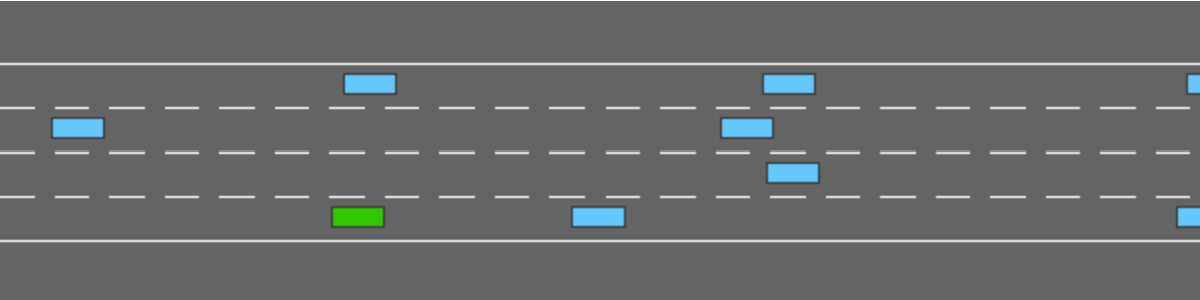
\includegraphics[width=0.73\textwidth]{images/chapter3/highway-env.png}
    \caption{highway-env仿真界面}\label{highway-env} % label 用来在文中索引
\end{figure}  

本文采用Highway-Env进行自动驾驶决策任务的设计,智能体(自我车辆)根据周围车辆的环境情况,获取环境反馈的奖惩值函数,通过执行决策行为间接控制车辆避障。因此,首先需要明确Highway-Env的状态、动作和奖励函数设计。

\subsubsection{Highway-Env的状态值设计}

在Highway-Env中有一系列的数据状态集合,针对自动驾驶避障问题,应当获取Kinetmatics的状态函数。Kinematics的状态是一张$V \times F$的表格,如表\ref{Kinetmatics状态表格}所示,$V$表示用户定义的车辆数量,$F$表示每个车辆的特征。第一列的$Vehicle$参数表示在当前画面中是否出现该车辆,如出现该车辆,则$Vehicle$值为1,否则为0。剩余的数值是车辆的坐标和速度,由于考虑的是自我车辆(ego-vehicle)的避障,所以环境中的其他车辆的坐标和速度均是相对于自我车辆的数值。

\begin{table}[htbp]
    % \vspace{13pt} % 调整图片与上文的垂直距离
    \caption{Kinetmatics状态表格}\label{Kinetmatics状态表格}
    \centering
    \renewcommand\arraystretch{1.5}
    \setlength{\tabcolsep}{7mm}{
    \begin{tabular}{|c|cccc|}
    \hline
    Vehicle     & \multicolumn{1}{c|}{$x$}  & \multicolumn{1}{c|}{$y$}  & \multicolumn{1}{c|}{$v_x$} & $v_y$ \\ \hline
    ego-vehicle & \multicolumn{1}{c|}{$x_{ego}$}   & \multicolumn{1}{c|}{$y_{ego}$}   & \multicolumn{1}{c|}{$v_{xego}$}      &  $v_{yego}$     \\ \hline
    vehicle 1   & \multicolumn{1}{c|}{$x_1$} & \multicolumn{1}{c|}{$y_1$} & \multicolumn{1}{c|}{$v_{x1}$}   & $v_{y1}$   \\ \hline
    vehicle 2   & \multicolumn{1}{c|}{$x_2$} & \multicolumn{1}{c|}{$y_2$} & \multicolumn{1}{c|}{$v_{x2}$}   & $v_{y2}$   \\ \hline
    $\dots$     & \multicolumn{4}{c|}{$\dots$}                                                           \\ \hline
    vehicle n   & \multicolumn{1}{c|}{$x_n$} & \multicolumn{1}{c|}{$y_n$} & \multicolumn{1}{c|}{$v_{xn}$}   & $v_{yn}$   \\ \hline
    \end{tabular}
    }
\end{table}

\subsubsection{Highway-Env的动作值设计}

DQN算法输入的是连续的状态,输出的是离散的动作。由于考虑的是决策问题,可以在决策之后增加一层低级的控制器,此处采用速度和转向控制器,使用P和PD控制器进行纵向和横向的解耦控制,使自我车辆能够以所需要的速度紧密跟随目标。关于低级控制器的部分在此不再赘述,表\ref{决策状态表格}表示了DQN的离散输出的决策所对应的动作量。动作值空间 A 的大小为5。

\begin{table}[htbp]
    % \vspace{13pt} % 调整图片与上文的垂直距离
    \caption{决策状态表格}\label{决策状态表格}
    \centering
    \renewcommand\arraystretch{1.5}
    \setlength{\tabcolsep}{7mm}{
    \begin{tabular}{|c|c|c|c|c|c|}
    \hline
    index  & 0  & 1  & 2  & 3  & 4  \\ \hline
    Action & 左转 & 保持 & 右转 & 加速 & 减速 \\ \hline
    \end{tabular}
    }
\end{table}

\subsubsection{Highway-Env的奖励函数设计}

选择合适的奖励函数决定了网络参数优化的方向,在Highway-Env的简单的仿真环境中,不需要在奖励函数中具体指定预期驾驶行为的每一个方面(例如行车的速度和与前车的安全距离),因为奖励函数不能由某个模型来确定。直接指定一个较为简单和直接的函数便能在学习中看到效果。

在自动驾驶避障问题中,通常关注车辆的速度和避免碰撞,所以奖励函数由速度项和碰撞项组成,如式\ref{highway_reward}所示,$v,v_{min},v_{max}$分别代表自我车辆的当前速度、最小速度和最大速度,$a,b$是速度项和碰撞项的两个系数。通过调整$a,b$两个系数能够使得智能体的优化方向更加偏向高速或偏向安全性。

\begin{equation}\label{highway_reward}
    R(s,a) = a\ \frac{v-v_{min}}{v_{max} - v_{min}} - b\ collision
\end{equation}

\subsection{网络结构设计} % 要出图,还有要介绍算法的学习过程。

针对Highway-Env的状态值、动作值和奖励函数设计,由于Highway-Env的决策环境较简单,网络结构设计两层全连接神经网络作为拟合行为值(Q值)函数的神经网络。如图\ref{DQN算法的决策器网络}所示,此过程为决策器网络的前向传播示意图,自我车辆与其他车辆的状态由\ref{3.1.1仿真环境}节的状态值获得,为了匹配DQN网络全连接层的输入要求,将表格中$V \times F$的二维数组压缩为一维数据,得到$1\times(V \times F)$的数据输入两层全连接神经网络。两层全神经网络之间使用$relu$函数激活,最终输出动作空间为5的决策动作。

\begin{figure}[htbp]
    \vspace{13pt}
    \centering
    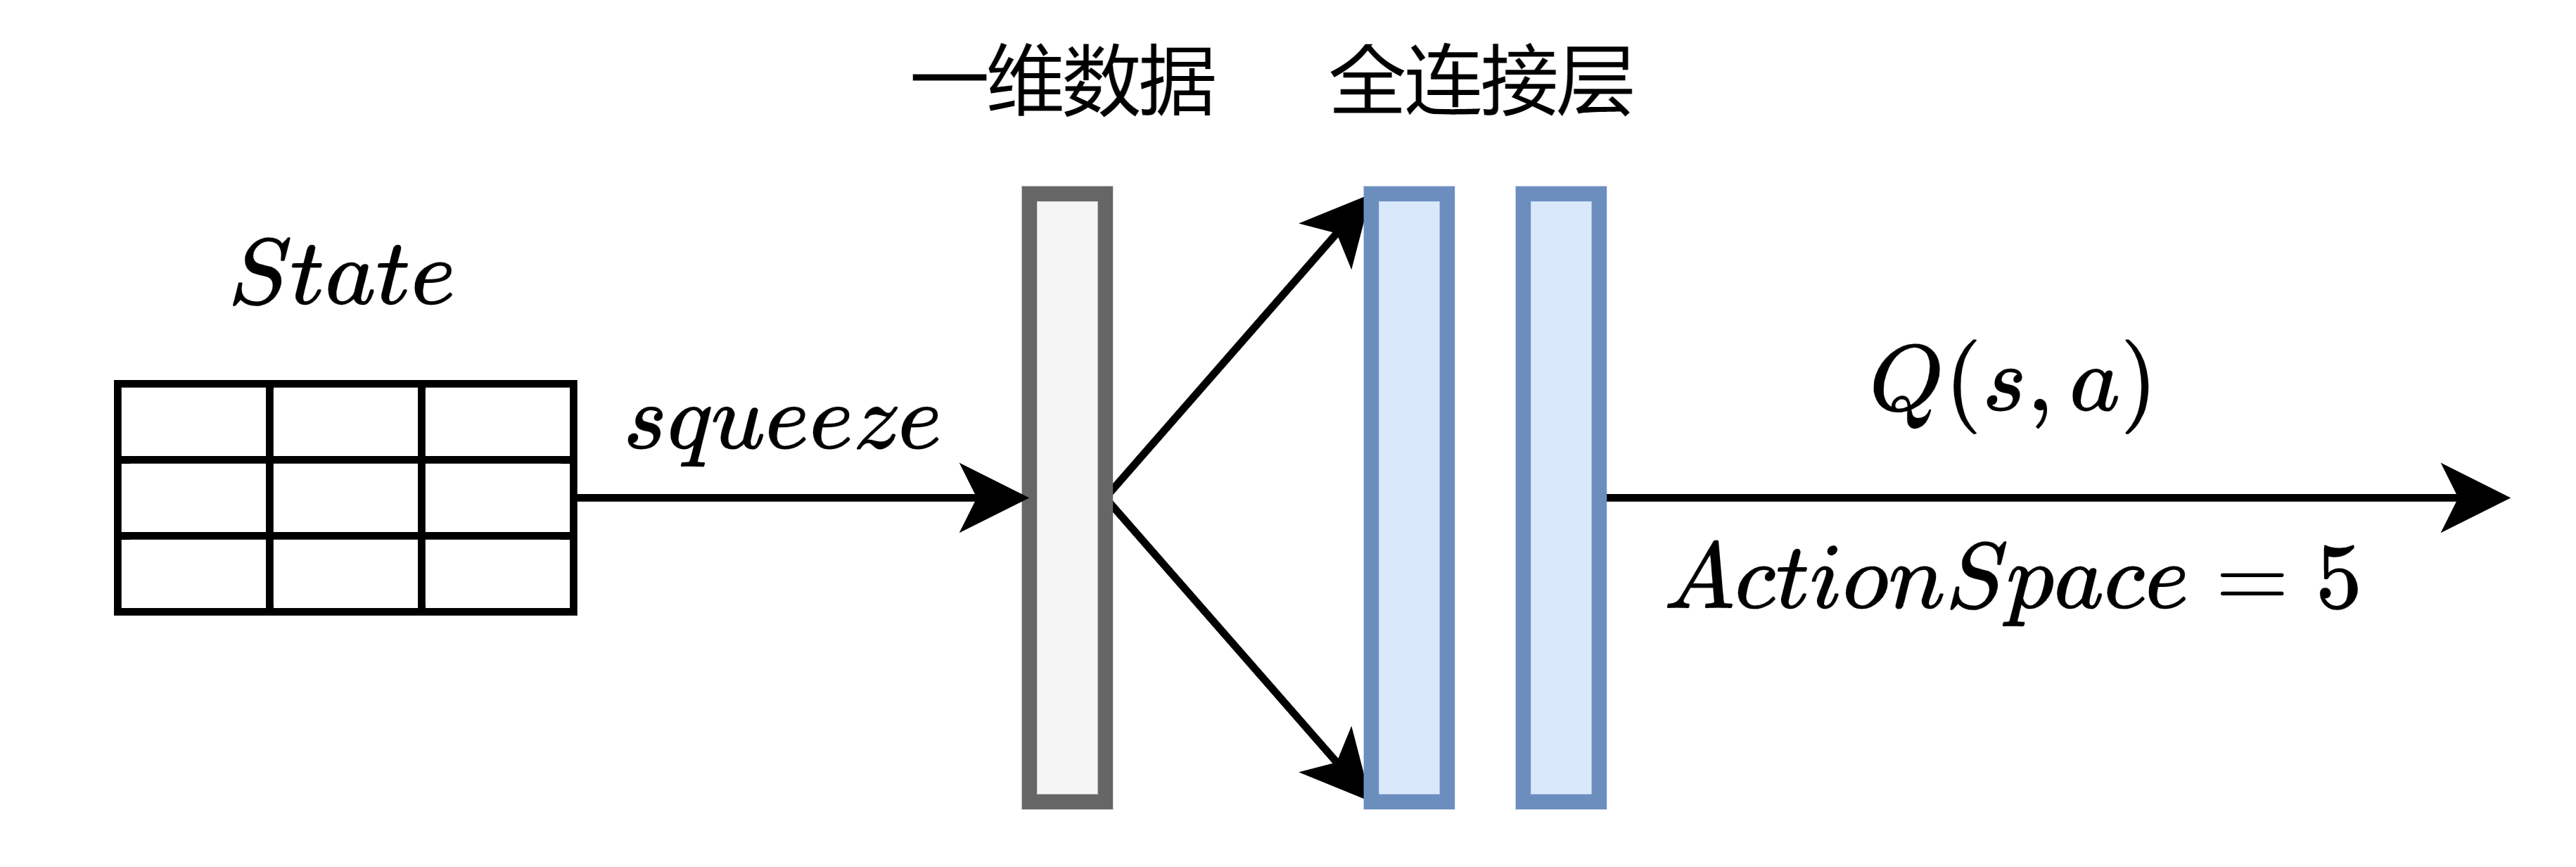
\includegraphics[width=0.73\textwidth]{images/chapter3/highway_decision.png}
    \caption{基于DQN算法的决策器网络}\label{DQN算法的决策器网络} % label 用来在文中索引
\end{figure}  

全连接层每一个结点都与上一层的所有结点相连,作用是将全连接层之前提取到的特征综合起来,最终输出行为值函数,以便后续环节的决策输出。根据前文DQN网络的相关研究,由于DQN网络需要实时的同智能体、环境交互,所以DQN网络一般采用较为简单的网络结构进行训练,其核心不在于网络结构的复杂程度,而在于算法的参数更新部分。和\ref{2.3DQN算法}节所示的DQN算法网络结构相比,Highway-Env获取的状态值是周围车辆相对于自我车辆的位置与速度,每个数据具有明确的指向性,所以不需要通过卷积层提取整体数据的特征,只采用两层的全连接层网络结构能够满足实验算法的准确度,又能保证运算速度和自动驾驶车辆决策动作的连贯。

\subsection{决策器的学习过程}

在决策器的网络结构设计结束后,决策器的算法需要根据\ref{2.3DQN算法}节所示的DQN算法进行构建。自动驾驶车辆首先获取当前的状态,每经过一个时间步,DQN算法都会对自动驾驶车辆的动作和网络结构参数进行更新。对于自动驾驶决策器而言,决策器的学习过程主要分为前向动作选取和反向数据更新两个部分。

\begin{figure}[htbp]
    \vspace{13pt}
    \centering
    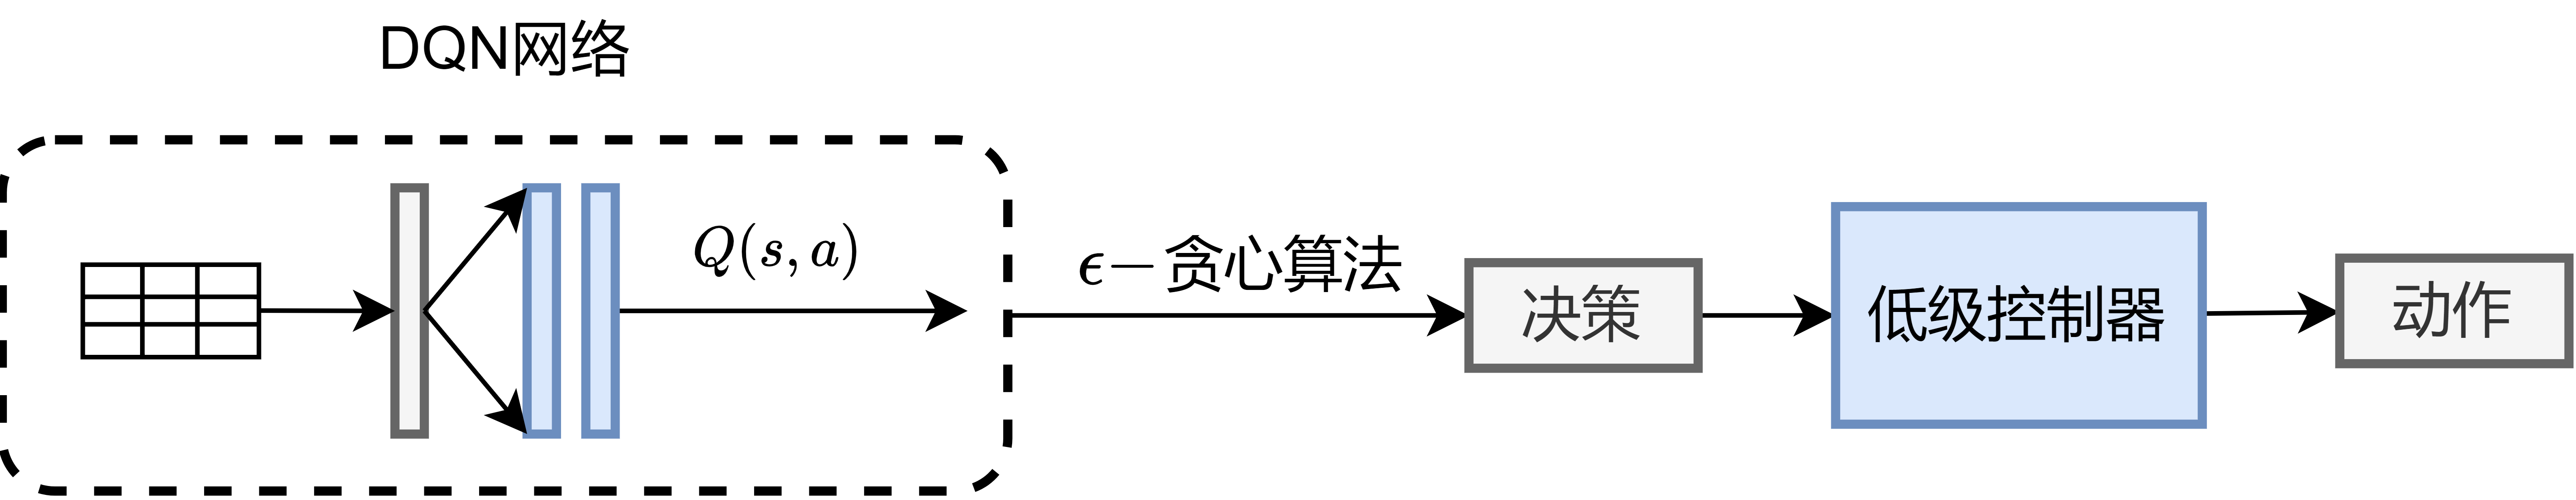
\includegraphics[width=0.85\textwidth]{images/chapter3/highway_forward.png}
    \caption{决策器前向动作选取}\label{决策器前向} % label 用来在文中索引
\end{figure}  

前向动作选取指的是在当前时刻,自动驾驶车辆将车辆当前的状态输入DQN的网络结构中,输出得到当前时刻车辆的决策动作。如图\ref{决策器前向}所示,DQN决策器网络输入自动驾驶车辆的当前状态,输出$1 \times 5$的行为值函数(Q值),在决策器学习过程中,采取$\epsilon-$贪心算法将行为值函数对应为选取的策略。每个时间步中,针对$1 \times 5$的行为值函数(Q值),以$\epsilon$概率随机选择任一随机动作,以$1-\epsilon$概率选择行为值函数最大的动作。$\epsilon$的值随着训练次数的增加而逐渐减小,在一定的训练次数后最终使得智能体选择行为值函数最大的决策动作。得到了行为值最大的决策动作,通过低级的控制器对应到Highway-Env的动作空间,从而使自动驾驶车辆完成对应的动作。

反向数据更新指的是DQN网络根据经验回放库中的数据,对DQN网络参数进行的更新。根据\ref{2.3DQN算法}节所示的DQN算法,DQN网络需要构建主网络($Q_{next}$)和TD网络($Q_{target}$),并且需要通过两者差值的平方作为损失函数进行反向传递。从经验回放库中随机采样得到数据,对每组数据的执行如下操作:

\begin{equation}
    \begin{aligned}
        q_{next} &= Q_{next}(s)\\
        q_{target} &= R(s,a) + \gamma \arg \max Q_{target}(s^{'})\\
        Loss &= MSELoss(q_{next},q_{target})\\
    \end{aligned}
\end{equation}
这里的更新方式借鉴了 Q-learning 的更新方式,最终的网络结构和参数更新通过Pytorch进行构建。

经过以上对Highway-Env仿真环境的状态值、动作值、奖励函数的说明和对DQN决策器详细的网络结构设计与分析,下一章节将以上述理论和具体实现方法作为依据,针对DQN及其改进算法在Highway-Env仿真环境中进行自动驾驶决策任务的实验验证。

\section{基于DQN算法的控制器设计} % 3.2 控制任务

\ref{3.1基于DQN算法的决策器设计}节基于DQN算法分析了自动驾驶任务决策器的设计思路,对于Highway-Env的仿真环境,输入车辆坐标等一系列抽象数据,输出运动控制的决策信息。基于端到端的方法要求直接从感知输入产生动作,当包含传感器信息输入的车辆状态维度进一步增加,直接对自动驾驶车辆的控制量(转矩与轮转角)进行离散后输出,不经过低级控制器对车辆进行实时控制,是基于DQN算法的控制器希望达成的目标。区别于Highway-Env的最小仿真环境,基于DQN算法的控制器设计需要对DQN网络的输入进行扩充,也需要更加真实的仿真环境与训练场景。

\subsection{仿真环境}

\begin{table}[htbp]
    % \vspace{13pt} % 调整图片与上文的垂直距离
    \caption{仿真模拟器对比}\label{仿真模拟器对比}
    \centering
    \renewcommand\arraystretch{1.5}
    \begin{tabular}{|c|c|c|c|c|c|}
    \hline
    Simulator   & 车辆动力学        & 多智能体       & 雷达、相机       & 真实数据导入       & 轻量级          \\ \hline
    CARLA\cite{Dosovitskiy17}       & $\checkmark$ & $\checkmark$ & $\checkmark$ & $\checkmark$ &              \\ \hline
    Metadrive\cite{li2021metadrive}   & $\checkmark$ & $\checkmark$ & $\checkmark$ & $\checkmark$ & $\checkmark$ \\ \hline
    Highway-Env\cite{highway-env} &              &              &              &              & $\checkmark$ \\ \hline
    \end{tabular}
\end{table}

MetaDrive 是一款高效的单车自动驾驶仿真模拟器\cite{li2021metadrive},和CARLA模拟器\cite{Dosovitskiy17}类似,Metadrive的状态、动作和奖励函数封装的较为完善,同时提供了较为准确的物理模型和多种传感器输入,优点是更加轻量级。多种仿真模拟器的对比如表\ref{仿真模拟器对比}所示:

Metadrive的仿真效果如图\ref{metadrive},相较于Highway-Env,它提供了更加具体的传感器输入和更加高维的观察输入,对于低级传感器(如RGB 摄像头、深度摄像头和激光雷达)可以放置在场景中的任何位置,参数可调节,同时,Metadrive还可以提供包括道路信息和附近车辆的速度和航向等高级场景信息作为状态量。本文采用Metadrive进行自动驾驶控制任务的设计。

\begin{figure}[htbp]
    \vspace{13pt} % 调整图片与上文的垂直距离
    \centering
    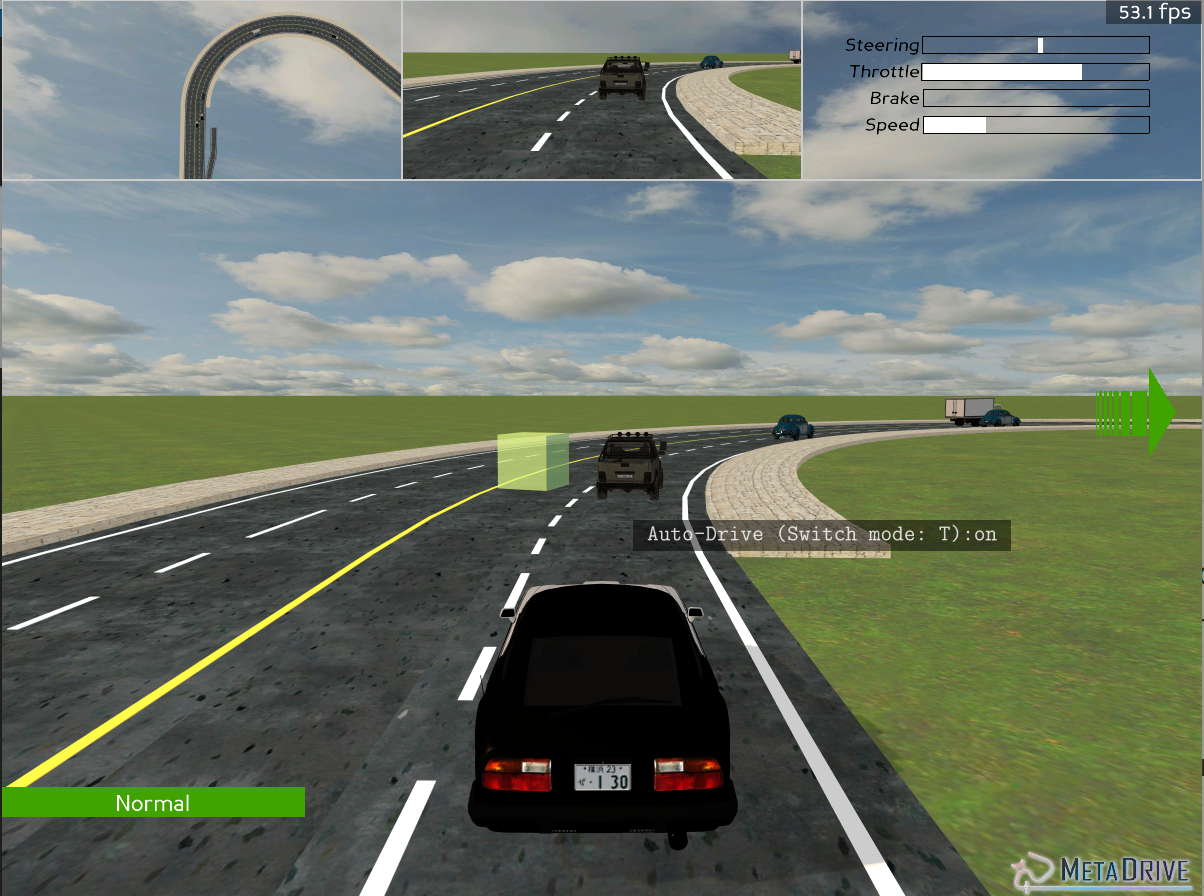
\includegraphics[width=0.73\textwidth]{images/chapter3/metadrive.png}%change
    \caption{metadrive仿真界面}\label{metadrive} % label 用来在文中索引
\end{figure}  

\subsubsection{Metadrive的状态值设计}

Metadrive提供一个状态向量,其中包含车辆导航任务所需的信息。状态向量由三部分组成:

(1) 车身状态

车身状态包括车辆当前的速度、转角、航向、控制量、横摆角速度和到边线的相对距离,这一部分包含了9个数据。

(2)导航信息

导航信息包含了引导车辆驶向目的地的信息,Metadrive首先计算车辆当前位置到目的地的路线,然后每组检查点以一定的间隔分散在整个路线上。到下一个检查点和下下一个检查点的相对距离和方向将作为导航信息给出,这一部分包含了10个数据。

(3)传感器信息

传感器信息设置为灰度相机的图像输入,周围信息通过$80\times80$的图像获取。针对于DQN算法,采用4帧$80\times80$的灰度图作为输入,这一部分包含了$4\times80\times80$个数据。

以上三部分数据在输入时都进行了归一化处理,都以$[0,1]$为区间进行了转换。

\subsubsection{Metadrive的动作值设计}

Metadrive接收标准化的动作作为输入进行车辆控制:
\begin{equation*}
    action = [steering, throttle]^{T} \in [-1,1]
\end{equation*}
在每个时间步长中,Metadrive将标准化的动作输入转换为轮转角$u_s$、发动机力$u_a$和制动力$u_b$。
\begin{equation*}
    \begin{aligned}
        u_s &= S_{max} steering\\
        u_a &= F_{max} max(0,throttle)\\
        u_b &= -B_{max} min(0,throttle)\\
    \end{aligned}
\end{equation*}
其中$S_{max}$是最大转向角,$F_{max}$是最大发动机力,$B_{max}$是最大制动力,通过这样的设计,每个智能体的动作空间总是固定的,这和标准化状态值设计是匹配的。

\subsubsection{Metadrive的奖励函数设计}

由于Metadrive所面对的环境更加复杂,故Metadrive的奖励函数也包含更多的部分,完整的奖励函数由以下三部分组成:
\begin{equation}
    R(s,a) = c_1 R_{driving} + c_2 R_{speed} + R_{termination}
\end{equation}

(1)驾驶奖励

\begin{equation*}
    \begin{aligned}
        &R_{driving} = (d_t - d_{t-1}) \times lateral\_factor\\
        &lateral\_factor = 1 - \frac{2\times lateral\_now }{lane\_width}
    \end{aligned}
\end{equation*}

其中$d_t$和$d_{t-1}$表示目标车辆在当前车道上连续两个时间步长的纵坐标,该奖励将鼓励智能体向前移动。$lateral\_factor$表示车辆是否远离了当前车道的中心,该奖励将鼓励智能体进行车道保持。

(2)速度奖励

$R_{speed} = v_t / v_{max}$,$v_t$和$v_{max}$表示当前速度与最大速度。该奖励将鼓励智能体尽可能接近$v_{max}$。

(3)终止奖励

$R_{termination}$是一组离散的奖惩函数,其包含了几种智能体可能的情况:
\begin{table}[htbp]
    \vspace{13pt}
    \centering
    \renewcommand\arraystretch{1.5}
    \begin{tabular}{|c|c|c|c|c|}
    \hline
    state & 车辆到达目的地 & 车辆驶出道路 & 车辆与其他车辆相撞 & 车辆撞到障碍物 \\ \hline
    cost  & +10.0   & -5.0   & -5.0      & -5.0    \\ \hline
    \end{tabular}
\end{table}

\subsection{网络结构设计} % 要出图,也要介绍算法的学习过程。

\begin{figure}[htbp]
    \vspace{13pt}
    \centering
    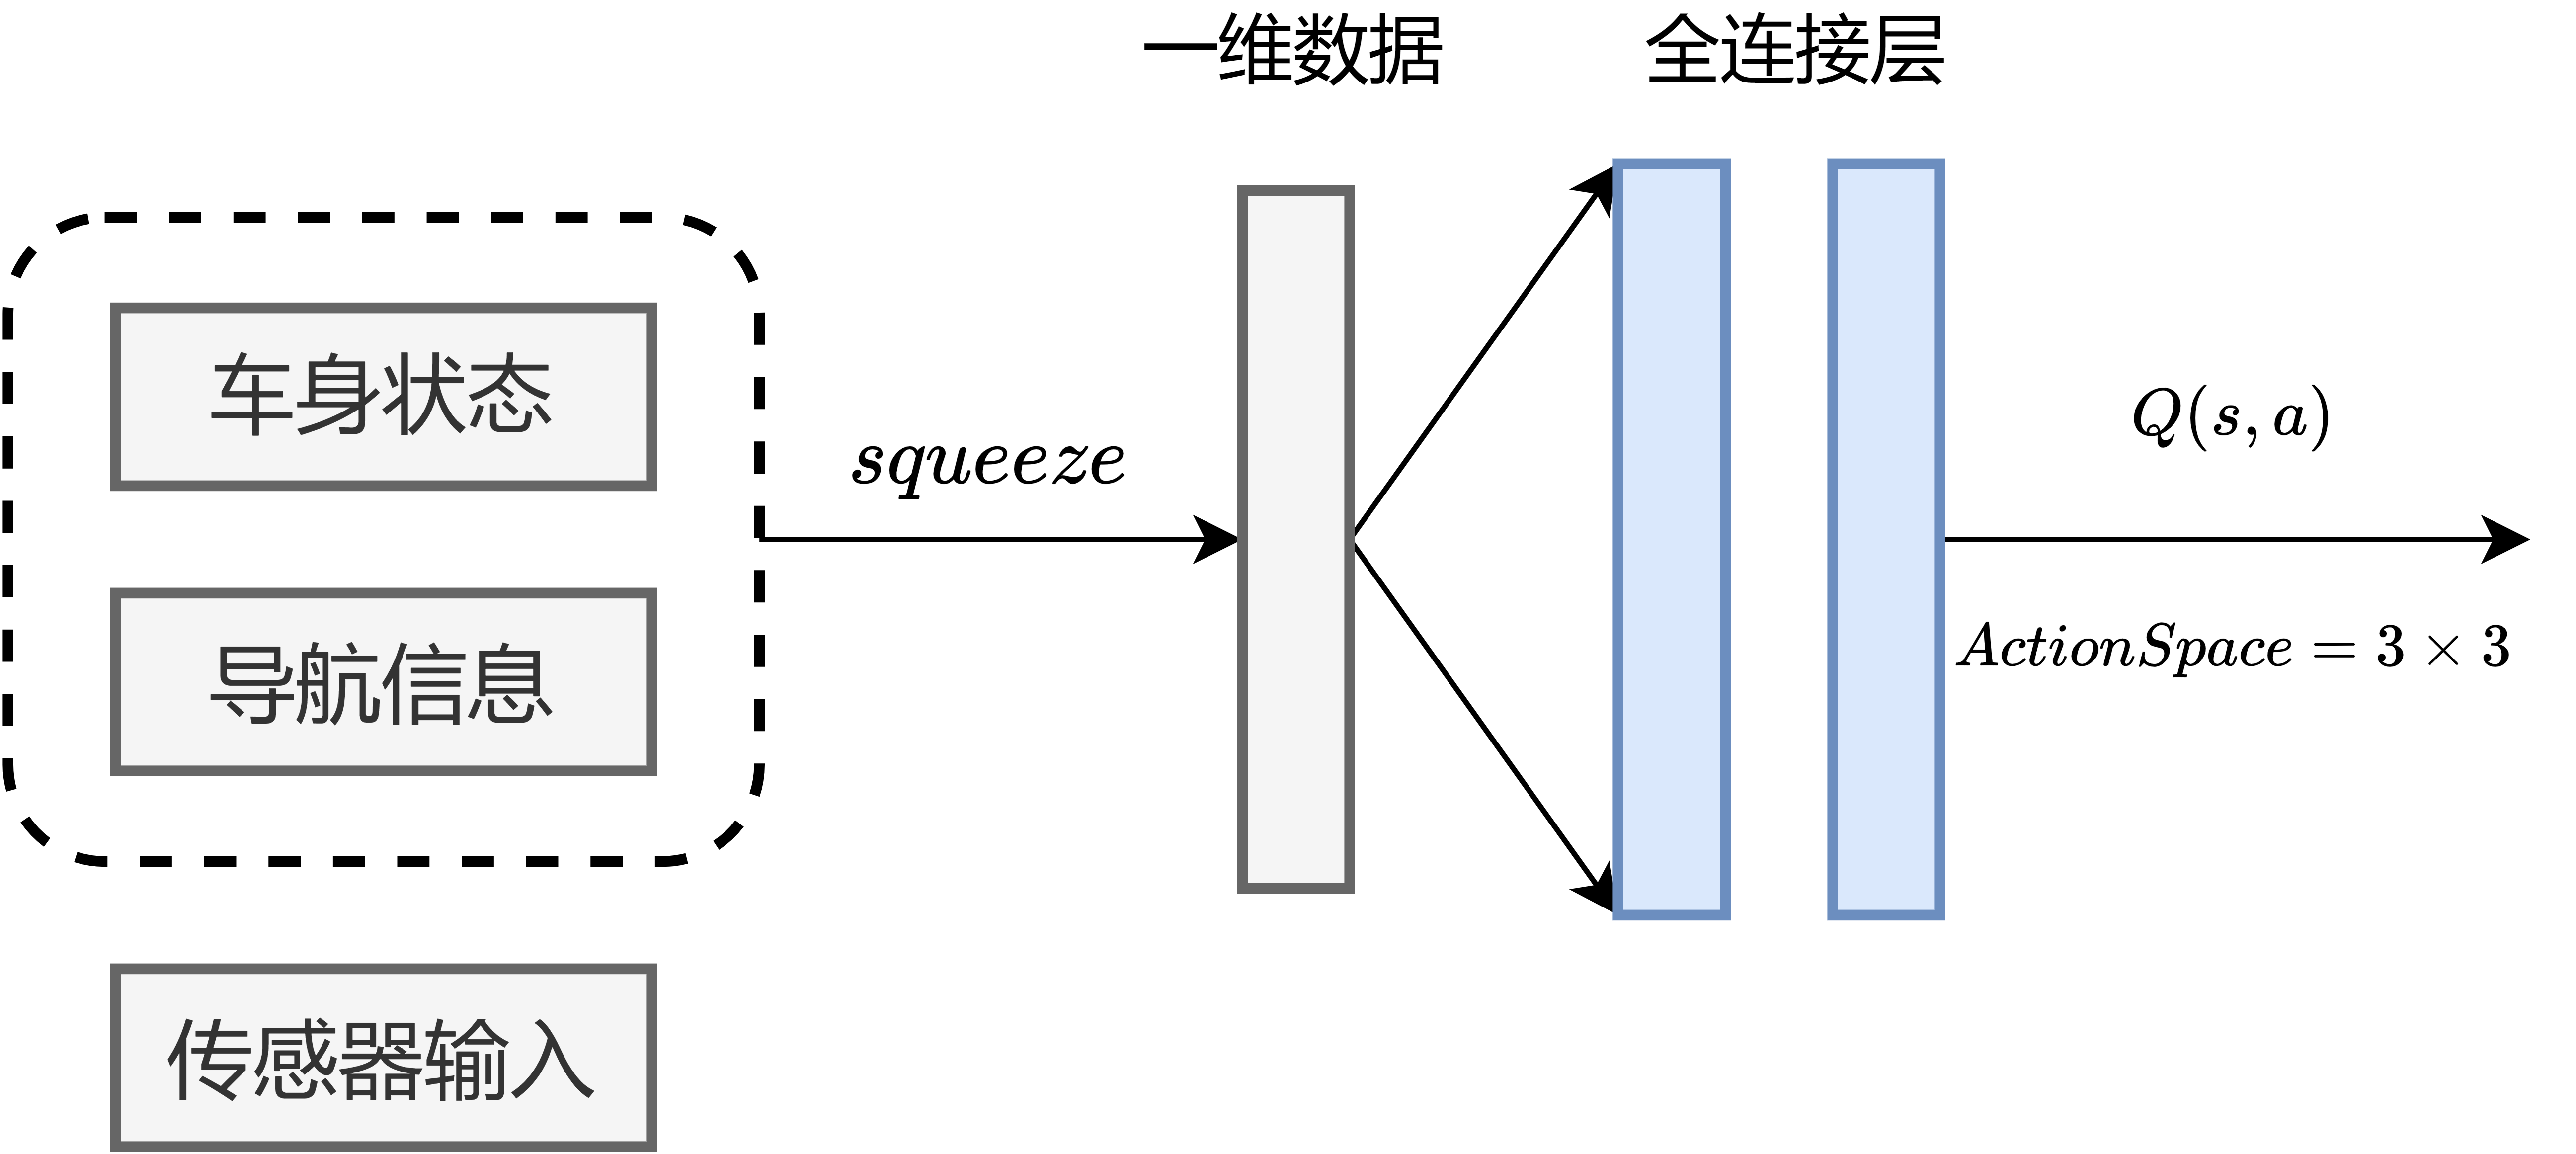
\includegraphics[width=0.73\textwidth]{images/chapter3/metadrive_control.png}
    \caption{基于DQN算法的控制器网络}\label{DQN算法的控制器网络} % label 用来在文中索引
\end{figure}  

Metadrive的状态量包括车身状态、导航信息和传感器信息,针对每个时间步长,车身状态和导航信息共包含19个数据,传感器信息包含$4\times80\times80=25600$个数据,因此前者与后者需要做出区分。网络结构设计需要明确网络结构与动作空间的大小,出于验证用途的考量,DQN的控制器设计预期实现使车辆在预定轨道上的循迹功能。参照Highway-Env的网络结构设计,仍采用两层全连接神经网络作为神经网络的结构,全连接层之间采用$relu$函数进行激活。在传感器信息方面,传感器获取周围车辆与道路信息,但是其获取的道路信息在车身状态与导航信息中已有体现,针对于车辆在预定轨道上的循迹功能,仅根据车身状态和导航信息便能依据全连接网络的综合能力完成相关任务,所以此时不将传感器信息作为网络结构的输入。具体的网络结构如图\ref{DQN算法的控制器网络}所示。

\begin{table}[htbp]
    % \vspace{13pt} % 调整图片与上文的垂直距离
    \caption{控制器动作空间}\label{控制器动作空间}
    \centering
    \renewcommand\arraystretch{1.5}
    \setlength{\tabcolsep}{7mm}{
    \begin{tabular}{|c|c|c|c|}
    \hline
    steering & -0.5 & 0 & 1   \\ \hline
    index    & 0    & 1 & 2   \\ \hline
    throttle & -0.5 & 0 & 0.5 \\ \hline
    index    & 0    & 1 & 2   \\ \hline
    \end{tabular}
    }
\end{table}

在动作空间的设计方面,动作空间分为$[steering, throttle]$两个分量,针对自动驾驶车辆的控制器而言,控制器要求在$50Hz-100Hz$的频率下做出响应,由于每个时间步长的间隔较短,且考虑到算力的限制,将连续的动作空间分为$3 \times 3$的均匀区间并对其进行编号,令$action\_index = 3 \times steering\_index + throttle\_index$,通过输出的索引确定输出的动作值。

\subsection{控制器的学习过程}

\begin{figure}[htbp]
    % \vspace{13pt}
    \centering
    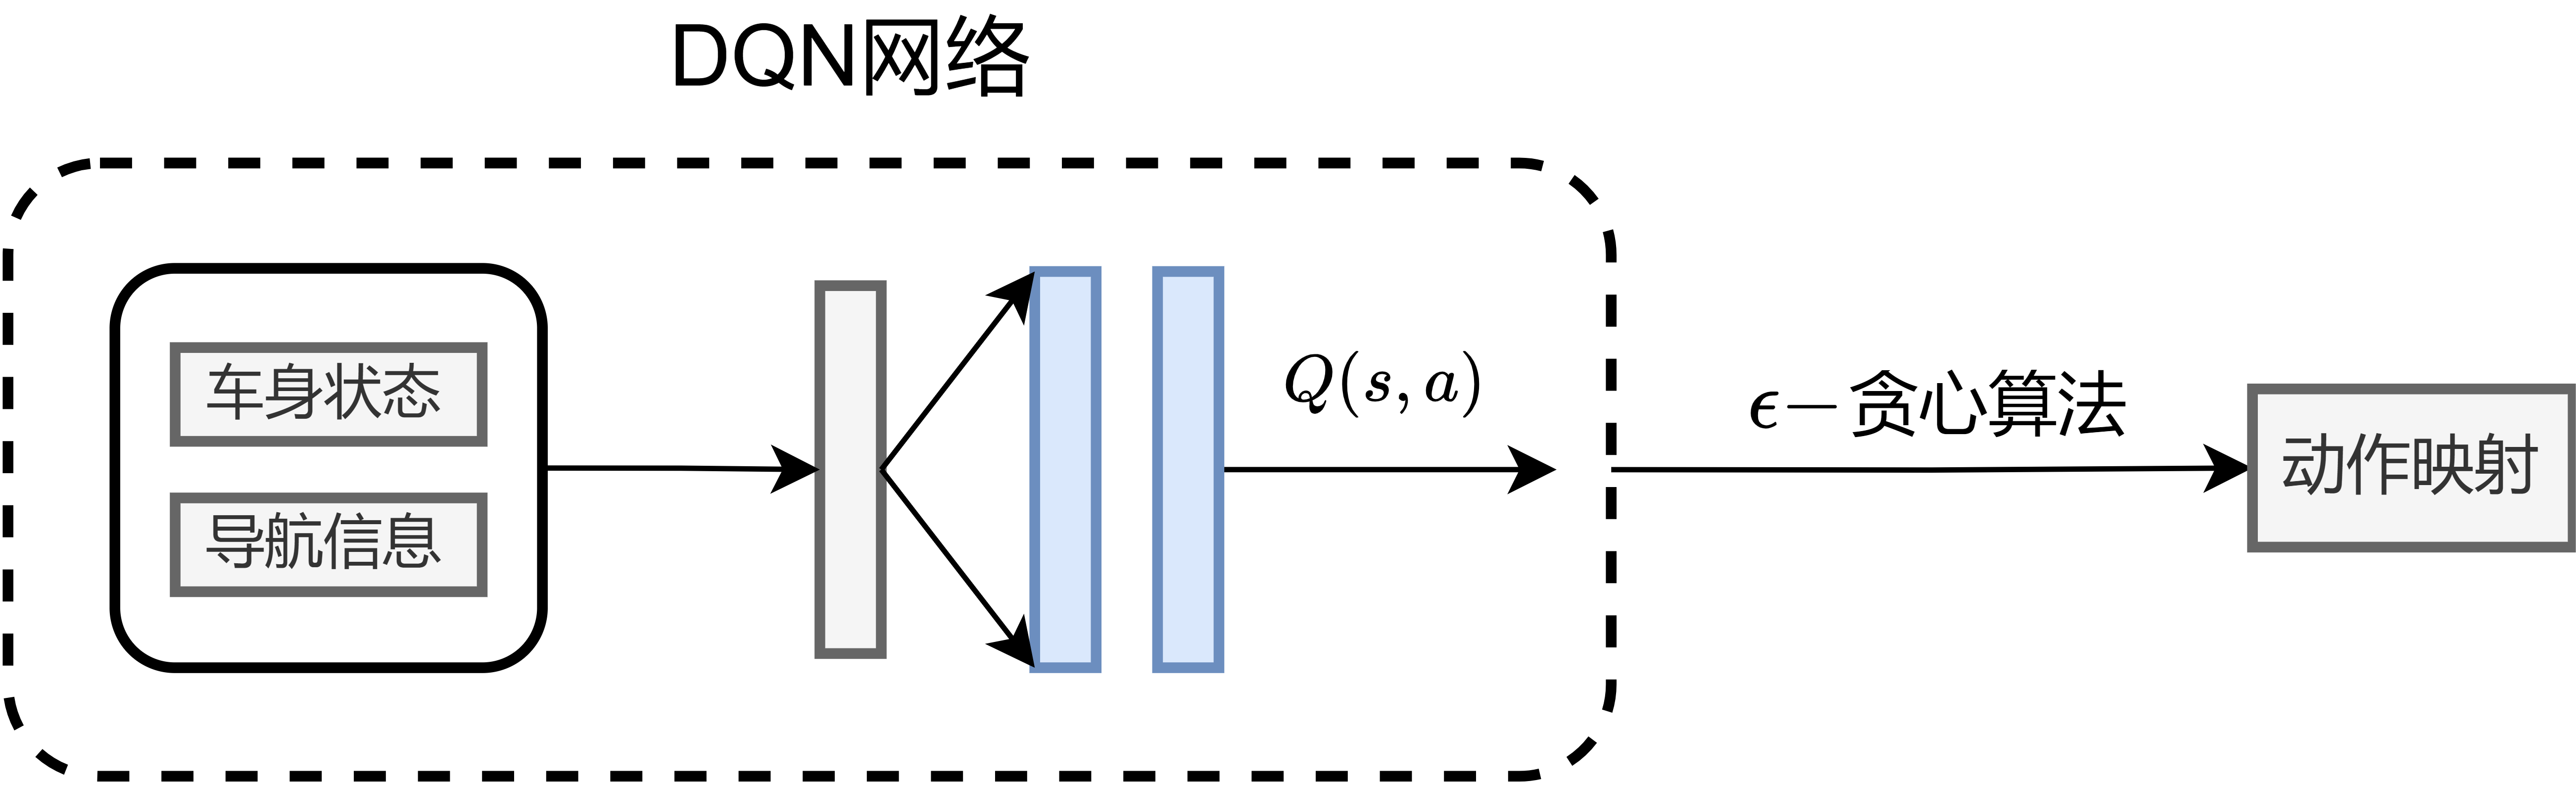
\includegraphics[width=0.85\textwidth]{images/chapter3/metadrive_forward.png}
    \caption{控制器前向动作选取}\label{控制器前向} % label 用来在文中索引
\end{figure}  

区别于Highway-Env的决策动作输出,Metadrive使用控制量进行端到端的直接输出,如图\ref{控制器前向}所示,DQN控制器网络输入自动驾驶车辆的车身状态与导航信息,输出$3 \times 3$的行为值函数(Q值),在控制器学习过程中,采取$\epsilon-$贪心算法将行为值函数对应为$action\_index$,并根据表\ref{控制器动作空间}映射到$[steering, throttle]$的实际控制量。尽管和决策器相比输入的信息含义并不相同,但通过全连接层的综合能力,能够将提取到的特征值进行综合,从而得到较为稳定的输出结果。

反向数据更新仍然是构建主网络($Q_{next}$)和TD网络($Q_{target}$),并通过两者差值的平方作为损失函数进行反向传递。从经验回放库中随机采样得到数据,对每组数据的执行如下操作:

\begin{equation}
    \begin{aligned}
        q_{next} &= Q_{next}(s)\\
        q_{target} &= R(s,a) + \gamma \arg \max Q_{target}(s^{'})\\
        Loss &= MSELoss(q_{next},q_{target})\\
    \end{aligned}
\end{equation}
这里的更新方式借鉴了 Q-learning 的更新方式,最终的网络结构和参数更新通过Pytorch进行构建。

\section{本章小结} % 3.3 本章小结

本章介绍了基于DQN及其改进型的自动驾驶避障算法设计,主要介绍了自动驾驶决策器和控制器应用的仿真环境,包括仿真环境的状态值、动作值和奖励函数的设计。在第2章算法研究的基础上,应用DQN及其改进算法,对自动驾驶决策器和控制器的网络结构设计和学习过程做了详细的分析与设计。

对于Highway-Env仿真环境,获取周围车辆相对于自我车辆的位置与速度信息,采用两层全连接神经网络拟合行为值(Q值)函数,使用DQN及其改进算法作为网络参数的更新策略,完成自动驾驶决策器的算法设计;对于Metadrive仿真环境,直接从感知输入产生动作,对自动驾驶车辆的控制量(转矩与轮转角)离散后输出,参照自动驾驶决策器的网络结构,获取车身状态与导航信息,完成车辆在预定轨道上的循迹功能。

至此,已经将基于DQN算法的决策器设计和基于DQN算法的控制器设计的理论和具体实现方法进行了详细的说明,后文将进行具体的实验对设计的算法进行验证。
